%
% File: Results.tex
% Author: Tengxiang Li
%
\chapter{Results and Discussion}
\label{chap:results}
\setlength{\parskip}{1em}
%

\section{Overview of Experimental Outcomes}
This chapter provides a multidimensional analysis of the empirical results gathered during our evaluation of gradient-based optimization, evolutionary computation, and direct random search paradigms. Specifically, we benchmark \textbf{Proximal Policy Optimization (PPO)}, \textbf{Evolution Strategies (ES)}, and \textbf{Augmented Random Search (ARS-V2)}. 

To ensure a rigorous evaluation of algorithmic robustness, these experiments were conducted under a strict ``zero-tuning'' protocol. In this framework, hyperparameters were held constant across all morphologies, forcing the algorithms to rely on their intrinsic exploration and stabilization mechanisms rather than environment-specific optimization. All agents were tested within a 3,000,000 timestep budget on the Apple M1 Pro architecture, utilizing the MuJoCo physics suite for high-dimensional continuous control tasks.


\section{Pillar 1: Asymptotic Performance}

\subsection{Conceptual Framework: Asymptotic vs. Cumulative Rewards}
In academic reinforcement learning, performance is typically judged through two distinct lenses:
\begin{enumerate}
    \item \textbf{Asymptotic Performance:} The steady-state episodic return achieved at the end of the training budget, calculated as the mean return of the final 10\% of training.
    \item \textbf{Cumulative Performance (AUC):} The Area Under the Curve of the reward trajectory, representing the total reward accumulated. A high AUC indicates a fast learner that reaches functional plateaus early.
\end{enumerate}

\subsection{Serial Execution Performance (1-Worker Baseline)}
In the serial (1-worker) baseline configuration, PPO established a dominant performance ceiling and superior cumulative learning across all benchmarks. As detailed in Table \ref{tab:1w_asymptotic}, PPO's asymptotic reward ($3588.88$) and cumulative AUC ($9.15 \times 10^9$) in \texttt{Walker2d-v4} were significantly higher than those achieved by both ES and ARS. This dual-metric dominance confirms that gradient-based updates not only reach a higher peak but also accumulate substantially more reward throughout the learning process under serial constraints.

Conversely, the low cumulative scores for ARS in \texttt{HalfCheetah-v4} ($4.33 \times 10^8$) highlight the representational limitations of static linear policies when deprived of the hyperparameter tuning necessary to navigate complex, non-terminating coordination tasks.

\begin{table}[h!]
\centering
\caption{Comparative Results for the 1-Worker Configuration Across Six Independent Seeds}
\label{tab:1w_asymptotic}
\begin{tabular}{@{}llrr@{}}
\toprule
\textbf{Environment} & \textbf{Algorithm} & \textbf{Asymptotic Score} & \textbf{Cumulative (AUC)} \\ \midrule
Hopper-v4 & PPO & 2117.15 & $6.31 \times 10^9$ \\
 & ES & 1439.80 & $2.70 \times 10^9$ \\
 & ARS & 1031.30 & $3.03 \times 10^9$ \\ \addlinespace
HalfCheetah-v4 & PPO & 3135.11 & $7.82 \times 10^9$ \\
 & ES & 2521.81 & $4.50 \times 10^9$ \\
 & ARS & 887.58 & $4.33 \times 10^8$ \\ \addlinespace
Walker2d-v4 & PPO & 3588.88 & $9.15 \times 10^9$ \\
 & ES & 1408.38 & $2.83 \times 10^9$ \\
 & ARS & 1019.76 & $2.45 \times 10^9$ \\ \addlinespace
Ant-v4 & PPO & 2346.96 & $4.98 \times 10^9$ \\
 & ES & 1426.09 & $3.35 \times 10^9$ \\
 & ARS & 724.14 & $2.49 \times 10^9$ \\ \bottomrule
\end{tabular}
\end{table}

\subsection{Parallel Execution Performance (4-Worker Scaling)}
Transitioning to a 4-worker distributed setup introduced a distinct performance-efficiency trade-off. While PPO’s asymptotic score improved in \texttt{Ant-v4} ($+25\%$), it saw a sharp decline in \texttt{Hopper-v4} ($-32\%$) and \texttt{HalfCheetah-v4} ($-52\%$). This degradation in both final reward and cumulative AUC suggests that partitioning the 2,048-step rollout into smaller 512-step sub-trajectories hampers advantage estimation by truncating the temporal context. This truncation likely introduces bias into gradient updates, leading to the observed instability.

Notably, parallel ES demonstrated superior resilience to distribution, achieving a higher terminal score than PPO in \texttt{HalfCheetah-v4} ($2429.54$ vs $1489.28$), as shown in Table \ref{tab:4w_asymptotic}. However, cumulative AUC indicates that ES utilized nearly the entire 3-million-step budget to achieve this score, whereas PPO reached its plateau significantly faster, maintaining superior sample efficiency despite the lower terminal return.

\begin{table}[h!]
\centering
\caption{Comparative Results for the 4-Worker Configuration Across Six Independent Seeds}
\label{tab:4w_asymptotic}
\begin{tabular}{@{}llrr@{}}
\toprule
\textbf{Environment} & \textbf{Algorithm} & \textbf{Asymptotic Score} & \textbf{Cumulative (AUC)} \\ \midrule
Hopper-v4 & PPO & 1443.25 & $3.72 \times 10^9$ \\
 & ES & 1700.53 & $3.04 \times 10^9$ \\
 & ARS & 1029.96 & $2.99 \times 10^9$ \\ \addlinespace
HalfCheetah-v4 & PPO & 1489.28 & $3.50 \times 10^9$ \\
 & ES & 2429.54 & $4.92 \times 10^9$ \\
 & ARS & 588.24 & $1.47 \times 10^8$ \\ \addlinespace
Walker2d-v4 & PPO & 3015.82 & $6.30 \times 10^9$ \\
 & ES & 1419.06 & $2.72 \times 10^9$ \\
 & ARS & 1016.14 & $2.51 \times 10^9$ \\ \addlinespace
Ant-v4 & PPO & 2944.47 & $4.18 \times 10^9$ \\
 & ES & 1658.56 & $3.73 \times 10^9$ \\
 & ARS & 705.88 & $2.52 \times 10^9$ \\ \bottomrule
\end{tabular}
\end{table}

\section{Figure Interpretation and Convergence Analysis}

The training curves illustrated in Figures \ref{fig:1worker} and \ref{fig:4worker} serve as a visual narrative of algorithmic behavior, highlighting the fundamental differences in convergence speed, variance, and response to distributed scaling.

\subsection{1-Worker Configuration: Peak Serial Efficiency}
In the 1-Worker configuration (Figure \ref{fig:1worker}), we observe PPO's rapid ascension. In morphologies like \texttt{Walker2d-v4} and \texttt{Ant-v4}, PPO reaches its performance plateau significantly earlier than its derivative-free counterparts. The shaded regions, representing $\pm 1$ standard deviation, remain relatively tight for PPO, suggesting high reliability across different random seeds. Conversely, ES exhibits a slower, more linear growth trajectory, while ARS frequently stagnates at low reward levels, particularly in \texttt{HalfCheetah-v4}.

\begin{figure}[htbp]
     \centering
     \begin{subfigure}[b]{0.45\textwidth}
         \centering
         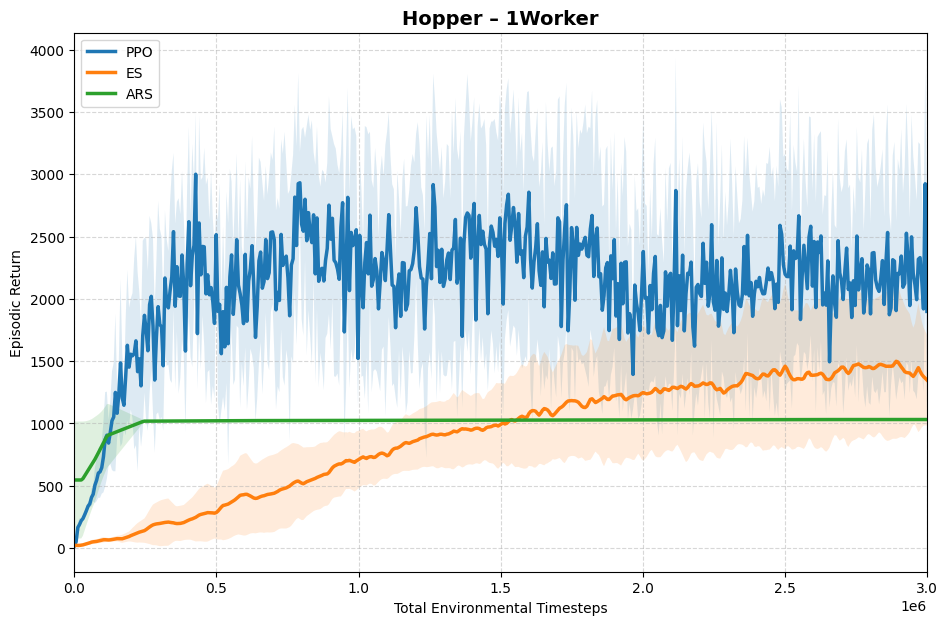
\includegraphics[width=\textwidth]{1-worker_Hopper_Reviewer_Fix.png}
         \caption{Hopper-v4}
     \end{subfigure}
     \hfill
     \begin{subfigure}[b]{0.45\textwidth}
         \centering
         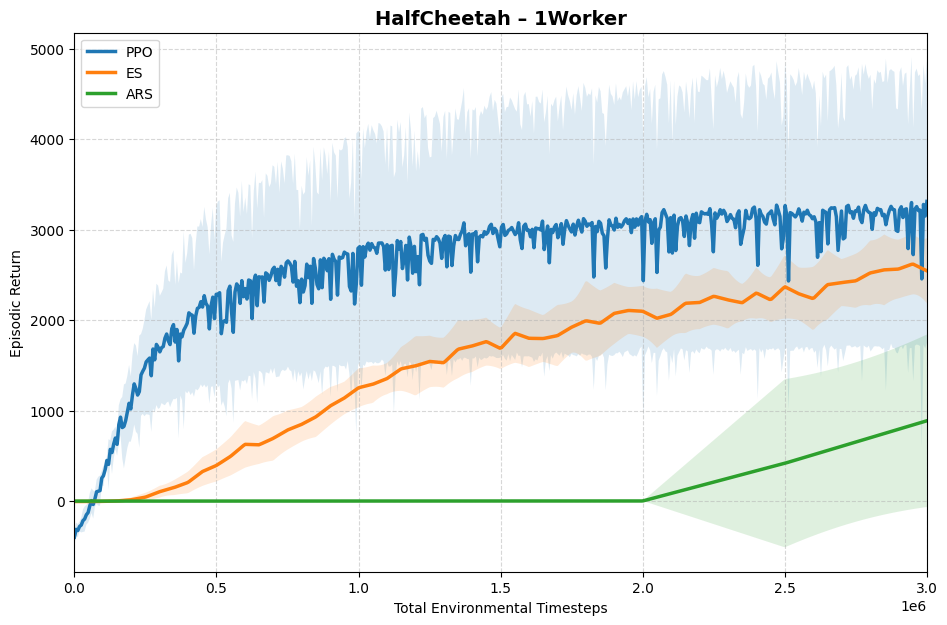
\includegraphics[width=\textwidth]{1-worker_HalfCheetah_Reviewer_Fix.png}
         \caption{HalfCheetah-v4}
     \end{subfigure}
     \vskip\baselineskip
     \begin{subfigure}[b]{0.45\textwidth}
         \centering
         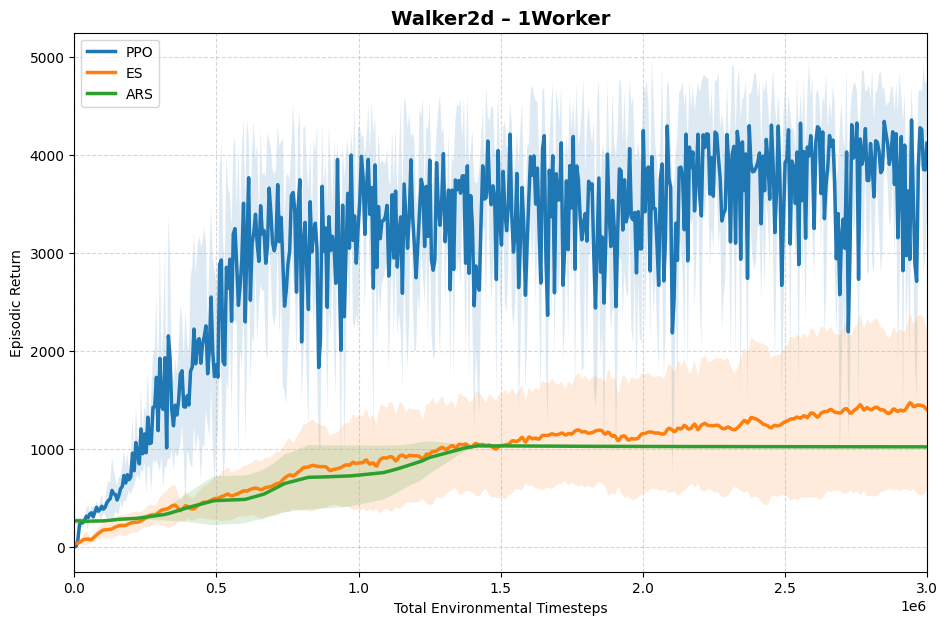
\includegraphics[width=\textwidth]{1-worker_Walker2d_Reviewer_Fix.png}
         \caption{Walker2d-v4}
     \end{subfigure}
     \hfill
     \begin{subfigure}[b]{0.45\textwidth}
         \centering
         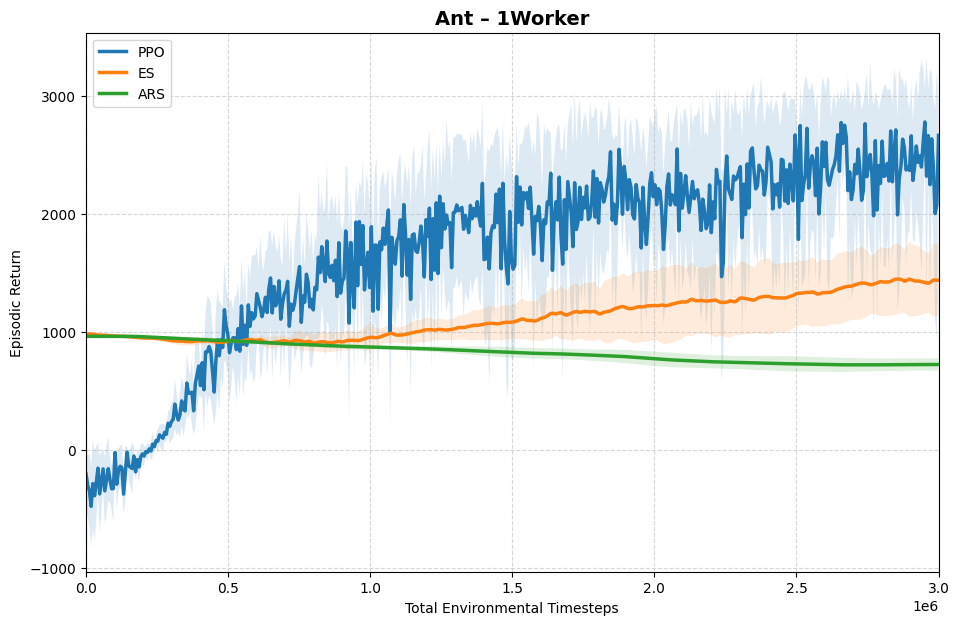
\includegraphics[width=\textwidth]{1-worker_Ant_Reviewer_Fix.png}
         \caption{Ant-v4}
     \end{subfigure}
     \caption{Training curves under 1-Worker configuration. The x-axis represents total environmental timesteps and the y-axis denotes episodic return. HalfCheetah-v4 is normalized by $5 \times 10^4$ steps/iteration for fair comparison. Shaded regions denote $\pm 1$ standard deviation ($n = 6$ seeds).}
     \label{fig:1worker}
\end{figure}

\subsection{4-Worker Configuration: Scaling and Instability}
The transition to 4-Worker scaling (Figure \ref{fig:4worker}) reveals a shift in algorithmic dominance. In \texttt{HalfCheetah-v4} (Figure \ref{fig:4worker}b), ES maintains its steady climb to eventually surpass PPO, which suffers a visible collapse in peak return compared to the serial case. This visualization grounds our earlier discussion on advantage estimation bias: the increased variance and lower mean for PPO in distributed settings are a direct consequence of fragmented rollout context.

\begin{figure}[htbp]
     \centering
     \begin{subfigure}[b]{0.45\textwidth}
         \centering
         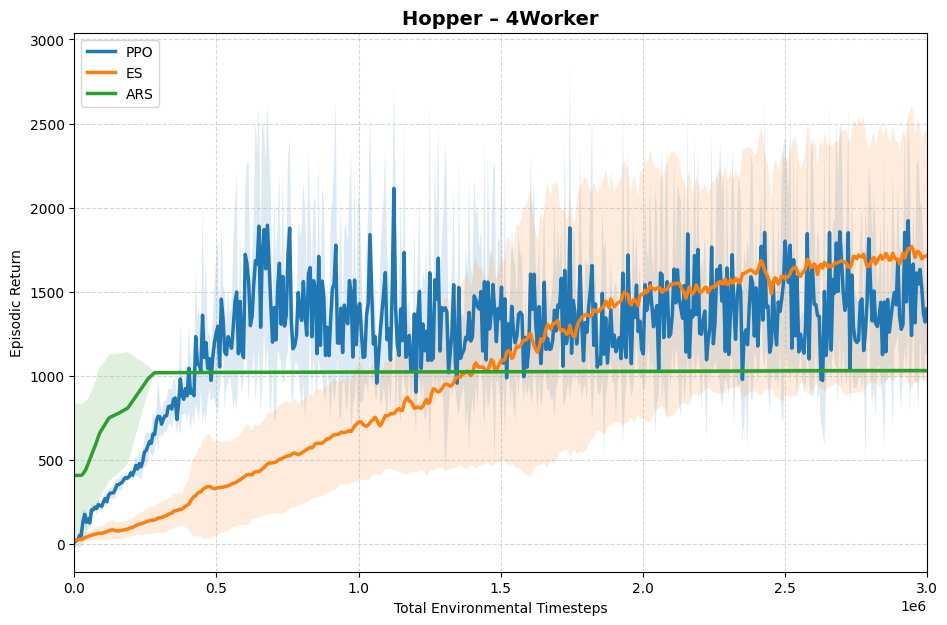
\includegraphics[width=\textwidth]{4-worker_Hopper_Reviewer_Fix.png}
         \caption{Hopper-v4}
     \end{subfigure}
     \hfill
     \begin{subfigure}[b]{0.45\textwidth}
         \centering
         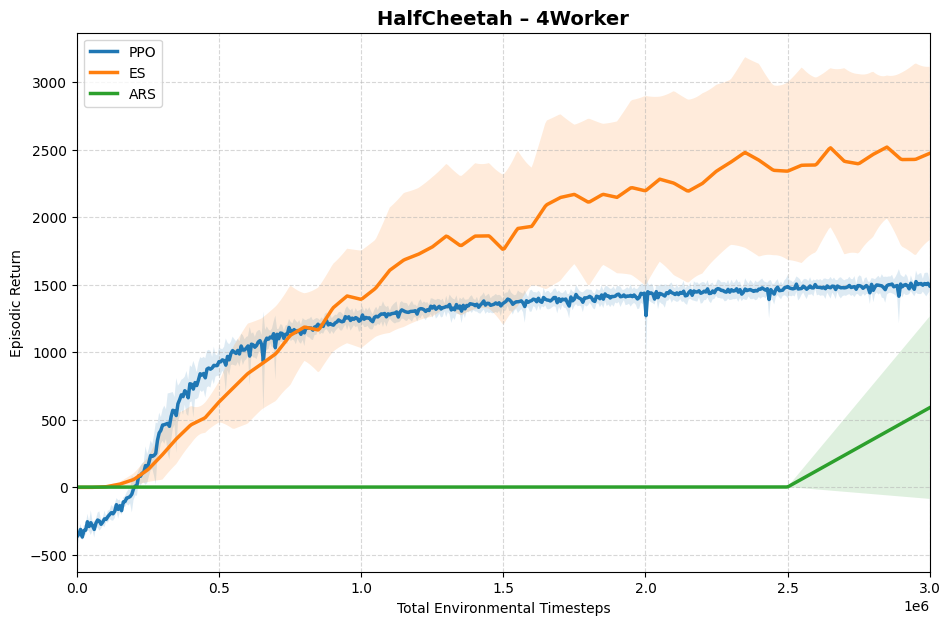
\includegraphics[width=\textwidth]{4-worker_HalfCheetah_Reviewer_Fix.png}
         \caption{HalfCheetah-v4}
     \end{subfigure}
     \vskip\baselineskip
     \begin{subfigure}[b]{0.45\textwidth}
         \centering
         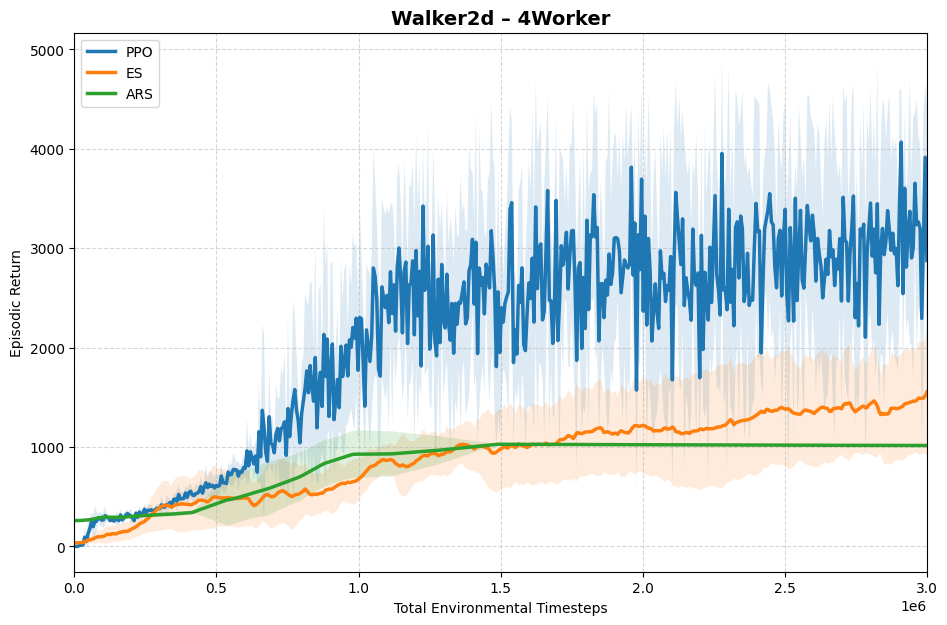
\includegraphics[width=\textwidth]{4-worker_Walker2d_Reviewer_Fix.png}
         \caption{Walker2d-v4}
     \end{subfigure}
     \hfill
     \begin{subfigure}[b]{0.45\textwidth}
         \centering
         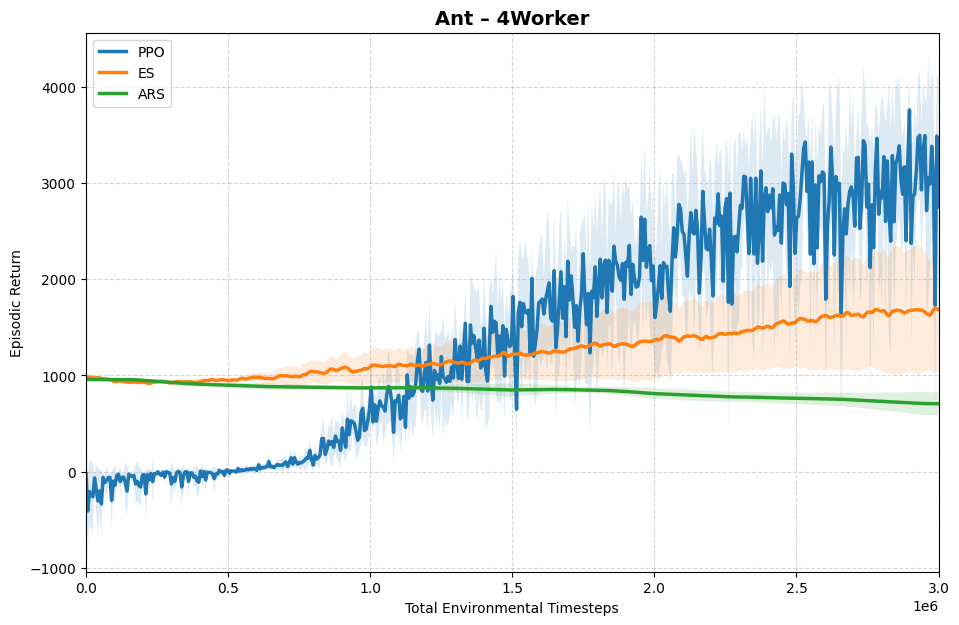
\includegraphics[width=\textwidth]{4-worker_Ant_Reviewer_Fix.png}
         \caption{Ant-v4}
     \end{subfigure}
     \caption{Training curves under 4-Worker configuration. The x-axis represents total environmental timesteps and the y-axis denotes episodic return. HalfCheetah-v4 is normalized by $5 \times 10^4$ steps/iteration for fair comparison. Shaded regions denote $\pm 1$ standard deviation ($n = 6$ seeds).}
     \label{fig:4worker}
\end{figure}

\section{Pillar 2: Efficiency and Scalability}

\subsection{Sample Complexity}
PPO consistently demonstrated the lowest sample complexity, leveraging backpropagated advantage estimates to extract a dense learning signal per timestep. As seen in the training curves (Figures \ref{fig:1worker} and \ref{fig:4worker}), PPO typically saturates its performance plateau within 1.0 to 1.5 million steps. 

In contrast, the rapid leveling off of ARS in \texttt{Ant-v4} reflects a premature performance ceiling (converging at a survival baseline of $\approx 700$) rather than true sample mastery. Under the strict zero-tuning constraint, PPO remains the only algorithm capable of extracting high behavioral knowledge with minimal environmental interactions.

\subsection{Temporal Efficiency: Thinking vs. Acting}
Despite higher sample requirements, derivative-free methods are substantially faster in wall-clock time, highlighting a ``thinking versus acting'' trade-off. PPO invests heavy computational overhead per update (gradients, advantage estimation, and multiple epochs) to extract maximum signal. 

Conversely, ARS and ES ``act'' rapidly with minimal per-iteration computation. As detailed in the Hardware Scalability Analysis (Table \ref{tab:hardware}), on the Apple M1 Pro, parallel ARS completed its entire training budget in a total time $T_4$ of just 5.7 minutes, whereas PPO required over 13 minutes for comparable saturation.

\subsection{Hardware Throughput and Scalability}
To quantify the computational efficiency of the underlying hardware backend, Table \ref{tab:hardware} evaluates the M1 Pro's performance across five metrics: Serial Time ($T_1$), Parallel Time ($T_4$), Parallel Speedup ($S$), Parallel Efficiency ($\text{Eff \%}$), and Steps Per Second ($\text{SPS}$).

\begin{table}[h!]
\centering
\caption{Hardware Scalability Analysis (Apple M1 Pro)}
\label{tab:hardware}
\begin{tabular}{@{}lrrrrr@{}}
\toprule
\textbf{Algorithm} & \textbf{$T_1$ (min)} & \textbf{$T_4$ (min)} & \textbf{Speedup ($S$)} & \textbf{Eff (\%)} & \textbf{SPS} \\ \midrule
PPO & 35.3 & 13.4 & $2.63\times$ & 65.8 & 3,729 \\
ES  & 17.8 & 7.5  & $2.39\times$ & 59.7 & 6,691 \\
ARS & 7.2  & 5.7  & $1.27\times$ & 31.6 & 8,838 \\ \bottomrule
\end{tabular}
\end{table}

PPO achieved the highest scalability with a $2.63\times$ speedup ($65.8\%$ efficiency), demonstrating that its gradient-based updates benefit significantly from distributed worker allocation on unified memory. 

Conversely, while ARS was the throughput leader---reaching 8,838 SPS, nearly $2.4\times$ the rate of PPO---it exhibited the lowest parallel efficiency ($31.6\%$). This is due to ARS's minimal serial training time (7.2 minutes); the computational load is so light that the Ray/Redis communication overhead becomes the primary bottleneck. These results validate the M1 Pro as a high-throughput workstation while highlighting the trade-off between raw execution speed (ARS) and efficient resource utilization (PPO).

\section{Pillar 3: Statistical Robustness}
To quantify the reliability of these results, the analysis focuses on convergence consistency, inter-seed variance (STD), and the Coefficient of Variation (CV) across six independent seeds. 
\begin{equation}
    CV = \frac{STD}{\text{Mean}} \times 100\%
\end{equation}

\begin{itemize}
    \item \textbf{Proximal Policy Optimization (PPO):} In the 1-worker configuration, PPO demonstrated the highest functional reliability in gait discovery. As evidenced by the asymptotic returns in Table \ref{tab:1w_asymptotic} and the stability metrics in Table \ref{tab:1w_stability}, PPO achieved the study's peak mean score ($3588.88$) in \texttt{Walker2d-v4} with a low CV of $6.53\%$, validating the stability of its clipping mechanism. However, Table \ref{tab:4w_stability} reveals a vulnerability to distribution; while the CV in \texttt{HalfCheetah-v4} narrowed to $3.93\%$, the mean score collapsed from $3135.11$ to $1489.28$. This suggests that while PPO becomes more ``consistent'' in its outcomes, it remains highly sensitive to temporal context fragmentation in distributed architectures.
    
    \item \textbf{Evolution Strategies (ES):} ES exhibited a unique trend where performance improved with scalability. Comparing Tables \ref{tab:1w_stability} and \ref{tab:4w_stability} shows that 4-worker settings raised mean scores in \texttt{Ant-v4} ($1426.09 \to 1658.56$) and \texttt{Hopper-v4} ($1439.80 \to 1700.53$). A broader search population acts as an implicit regularizer, smoothing the fitness landscape. However, the CV in \texttt{Hopper-v4} rose to $44.14\%$ in the 4-worker setup, suggesting that while parallel exploration raises the performance ceiling, the stochastic nature of evolutionary steps maintains a wide distribution of outcomes.
    
    \item \textbf{Augmented Random Search (ARS):} While ARS-V2 mathematically achieved the lowest CV in tasks like \texttt{Walker2d-v4} ($0.47\%$), this reflects a ``stable failure'' state. Rather than reliably discovering functional gaits, the agent consistently converged to a sub-optimal, static survival baseline. The algorithm's true fragility under the zero-tuning protocol is most apparent in \texttt{HalfCheetah-v4}, where the CV exceeded $100\%$ in both configurations. This extreme variance reflects a bimodal distribution of outcomes—either immediate failure or negligible progress. Ultimately, enforcing a fixed step size ($\alpha = 0.03$) severely handicapped ARS's ability to adapt to varying reward scales, confirming that its reliability is critically dependent on environment-specific hyperparameter optimization.
\end{itemize}

\begin{table}[htbp]
\centering
\caption{Stability Metrics (1-Worker Baseline)}
\label{tab:1w_stability}
\begin{tabular}{@{}lrrrrrr@{}}
\toprule
\textbf{Environment} & \multicolumn{2}{c}{\textbf{PPO}} & \multicolumn{2}{c}{\textbf{ES}} & \multicolumn{2}{c}{\textbf{ARS}} \\
\cmidrule(lr){2-3} \cmidrule(lr){4-5} \cmidrule(lr){6-7}
 & \textbf{CV (\%)} & \textbf{STD} & \textbf{CV (\%)} & \textbf{STD} & \textbf{CV (\%)} & \textbf{STD} \\ \midrule
Hopper-v4 & 32.20 & 681.67 & 36.85 & 530.55 & 1.01 & 10.42 \\
HalfCheetah-v4 & 45.83 & 1436.95 & 14.52 & 376.96 & 107.35 & 952.86 \\
Walker2d-v4 & 6.53 & 234.43 & 60.59 & 853.35 & 0.59 & 6.00 \\
Ant-v4 & 18.78 & 440.77 & 19.96 & 284.72 & 7.10 & 51.40 \\ \bottomrule
\end{tabular}
\end{table}

\begin{table}[htbp]
\centering
\caption{Stability Metrics (4-Worker Configuration)}
\label{tab:4w_stability}
\begin{tabular}{@{}lrrrrrr@{}}
\toprule
\textbf{Environment} & \multicolumn{2}{c}{\textbf{PPO}} & \multicolumn{2}{c}{\textbf{ES}} & \multicolumn{2}{c}{\textbf{ARS}} \\
\cmidrule(lr){2-3} \cmidrule(lr){4-5} \cmidrule(lr){6-7}
 & \textbf{CV (\%)} & \textbf{STD} & \textbf{CV (\%)} & \textbf{STD} & \textbf{CV (\%)} & \textbf{STD} \\ \midrule
Hopper-v4 & 6.06 & 87.44 & 44.14 & 750.69 & 1.47 & 15.14 \\
HalfCheetah-v4 & 3.93 & 58.58 & 31.05 & 866.04 & 114.87 & 675.70 \\
Walker2d-v4 & 17.45 & 526.24 & 36.12 & 512.57 & 0.47 & 4.73 \\
Ant-v4 & 6.11 & 179.97 & 37.46 & 621.23 & 16.90 & 119.28 \\ \bottomrule
\end{tabular}
\end{table}

\section{Pillar 4: Qualitative Gait Analysis}
While the preceding sections quantified ``how much'' each agent learned, this section investigates the physical strategies adopted by trained policies. This qualitative analysis reveals a notable \textit{Integrity Gap} between numerical rewards and physical plausibility.

\subsection{The Survival Bonus Trap and Local Optima}
A recurring theme was the exploitation of the survival bonus, which incentivizes standing still over forward locomotion. In \texttt{Ant-v4}, ARS reached scores near $1,000$ by remaining almost immobile—the ``Lazy Ant'' phenomenon. 

PPO exhibited an even more extreme version of this exploitation; in 1-worker configurations, it occasionally converged to a non-moving state that yielded rewards of approximately $2,000$—double that of the ``Lazy'' ARS—simply through superior optimization of the survival mechanism. However, in 4-worker settings, PPO's representational capacity allowed it to transcend these mechanics, reaching rewards exceeding $3,000$.

This was equally pronounced in \texttt{Hopper-v4}, where ARS converged to a $\sim 1,000$-reward local optimum by balancing in place. Dense survival rewards often bias agents toward static stability. Replicating the ablation study to force forward progress revealed an intriguing paradox: while the ARS-trained Hopper developed a functional, forward-moving gait, its episodic return remained anchored near $1,000$. 

This encapsulates the \textbf{Efficiency-Integrity Gap}: identical scalar rewards can represent entirely disparate physical realities. One policy is a static balancing act exploiting mechanics; the other is a viable locomotion strategy. Relying solely on scalar metrics masks this fundamental behavioral divergence.

\subsection{Morphological Exploitation and Reward Hacking}
Beyond passive strategies, agents discovered behavioral ``hacks'' that maximized reward by exploiting physics-engine artifacts rather than learning biologically plausible locomotion:

\begin{itemize}
    \item \textbf{The Upside-Down Cheetah (PPO):} In \texttt{HalfCheetah-v4}, PPO achieved high returns by flipping onto its back and sliding forward. Because the reward function emphasizes forward velocity, sliding along the spine minimized joint friction and control penalties. While biomechanically unrealistic, this behavior is mathematically optimal under the reward formulation.
    
    \item \textbf{The Jittering Evolution (ES):} In \texttt{Walker2d-v4}, ES reached competitive reward levels through a high-frequency jittering motion. The policy exploited contact dynamics by inducing rapid joint oscillations to generate forward momentum. While effective in simulation, such a strategy would cause immediate structural failure in a physical robot.
    
    \item \textbf{Functional Divergence (PPO in Walker2d):} In contrast to exploitative hacks, PPO demonstrated two distinct, high-performing solutions ($\sim 3,000$ reward) in \texttt{Walker2d-v4}: a conventional alternating bipedal stride and a dynamic hopping strategy. This suggests that gradient-based optimization can effectively explore and converge upon multiple viable optima within the policy landscape.
\end{itemize}

\section{Summary}

This chapter presented a multi-dimensional evaluation of PPO, ES, and ARS across four analytical pillars, leveraging the Apple M1 Pro's ARM-based architecture to examine the interaction between algorithmic theory and hardware constraints. The investigation produced several key insights:

\begin{itemize}
    \item \textbf{Asymptotic Performance and Stability:} PPO established the performance ceiling in serial (1-Worker) configurations, achieving the highest reward levels with comparatively low variance. However, the transition to 4-worker parallelization induced a measurable algorithmic shift. While PPO exhibited increased volatility and performance degradation in certain environments due to trajectory fragmentation, ES demonstrated a notable parallel breakthrough, surpassing PPO in the high-dimensional \texttt{HalfCheetah-v4} task.
    
    \item \textbf{The Efficiency--Throughput Trade-off:} A pronounced contrast emerged between sample complexity and temporal throughput. ARS proved to be the throughput leader, achieving 8,838 Steps Per Second (SPS) and completing full training cycles in under six minutes. Nevertheless, its iterations were less information-dense than PPO's gradient-driven updates. PPO remained the most sample-efficient algorithm, though it incurred substantially greater wall-clock time per optimization step due to the computational overhead of backpropagation.
    
    \item \textbf{Hardware Scalability on Unified Memory:} The Apple M1 Pro's unified memory architecture delivered the greatest parallel benefit to PPO, which achieved the highest Parallel Speedup ($S = 2.63\times$). In contrast, the lightweight computational footprint of ARS rendered it communication-bound in distributed configurations, where the inter-process overhead of Ray/Redis reduced the relative gains from additional CPU cores.
    
    \item \textbf{Behavioral Fidelity and the Integrity Gap:} The qualitative analysis exposed a significant gap between numerical optimization and physical reality. Although ES and ARS achieved competitive numerical rewards, they frequently relied on ``reward hacks" such as survival-based stasis (the ``Lazy Ant'' strategy) or high-frequency joint jittering that exploited simulator dynamics. PPO was the only algorithm to consistently produce stable locomotion, suggesting that gradient-based precision is instrumental in maintaining mechanical plausibility.
\end{itemize}

\medskip

\noindent In summary, derivative-free methods such as ES and ARS offer compelling advantages in temporal throughput and parallel scalability on modern silicon. However, they lack the representational density necessary for high-fidelity continuous control without extensive tuning. For complex robotic tasks, the optimization precision of PPO remains essential to balance survival incentives, forward velocity, and physical plausibility.

\clearpage
\null 
\clearpage